\documentclass{article}
 
\usepackage{color}
\usepackage{listings}
\usepackage{graphicx}
\usepackage{subfig}

\definecolor{MyYellow}{rgb}{1,1,0.8}
 
\lstset{language=Matlab,backgroundcolor=\color{MyYellow},basicstyle=\footnotesize,numberstyle=\footnotesize,numbers=left,stepnumber=1,numbersep=5pt,breaklines=true,frame=lines,tabsize=2}
 
\author{Ruurd Moelker \and Jan Paul Posma}
\date{\today}
\title{Signalen \& Systemen \\Practicum 3}

\begin{document}
\maketitle
 
\section{Opgave 1.1}
$hh = conv([1 -2*cos(0.44*pi) 1], [1 -2*cos(0.7*pi) 1])$
$hh = [1 0,8008 1,5594 0,8008 1]$
$freqz( conv([1 -2*cos(0.44*pi) 1], [1 -2*cos(0.7*pi) 1]) )$



\section{Opgave 1.2}
$xx = $

\section{Opgave 1.3}
In figuur .. staat het signaal voor de filter. In figuur .. staat het gefilterde signaal.

n>5 --> $10*cos(0.3*pi*n)$ met nog een factor uit 1.1
De amplitude behorende bij het formule van het gefilterd signaal is een verdubbeling van de amplitude 5 in het invoer signaal. Dit is ook te zien in figuur .. omdat bij 0.3 een versterking van 2 staat.

\section{Opgave 1.4}

\section{Opgave 2.1}
$L = 10$
$hh2 = 2/L * cos( \omega*n)$ waarbij $0\leq n \leq L$

Een plot van de gain filter staat in figuur .. .

De invloed van het bandpass filter op signaal xx staat in figuur ...
De sterkte van het filter op de frequentie $0.3\pi$  = 0,28.
De sterkte van het filter op de frequentie $0.44\pi$  = 1,1.
De sterkte van het filter op de frequentie $0.7\pi$  = 0,28.

\section{Opgave 2.2}

Om de frequentie waarden te vinden die in de band zitten gebruiken we voor de verschillende waarden van L achtereenvolgens:
$nn2 = (0:19);$
$hh2 = 2/L* cos( \hat{\omega}*nn2)$
$length(find(abs(H/max(H)) > 1/sqrt(2)))) / length(W)$


De gevonden breedte horende bij de ingevoerde waarde van L zijn als volgt:
$L=10 --> 0,164*pi$
$L=20 --> 0,086*pi$
$L=40 --> 0,043*pi $


\section{Opgave 2.3}
$hh = 2/L*cos(w*(0:(L-1))); 
[H,W] = freqz(hh); 
min(min(abs(H(0.7*length(H): length(H))) <= 0.1), (min(abs(H(1:0.3*length(H))) <= 0.1) == 1))$

\section{Opgave 2.4}
\begin{figure}[h]
  \centering
 	\subfloat[][x[n]]{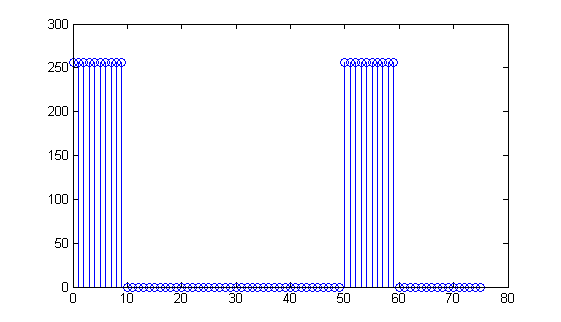
\includegraphics[width=0.4\textwidth]{content/2xx.png}}
	\subfloat[][w[n]]{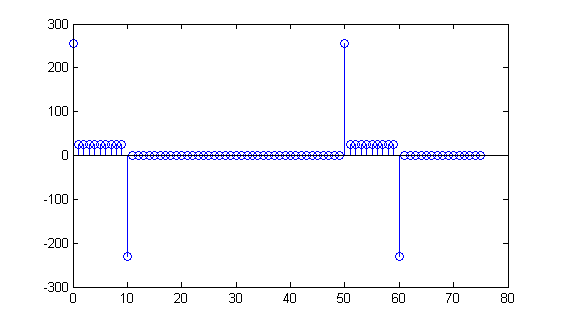
\includegraphics[width=0.4\textwidth]{content/2ww.png}}
  \caption{Stemplot van x en w over het interval [0..75]}
  \label{fig:opgave2}
\end{figure}

\section{Opgave 3}
Het matlab commando $length()$ geeft de lengte van een signaal. Voor x[n] is deze lengte 101 en voor w[n] is de lengte 102. De lengte van de convolutie wordt inderdaad bepaald door $length(xx)+length(bb)-1$ waarbij bb de vector met co\"efficienten is, in dit geval [1, -0.9], dus lengte 2.

\section{Opgave 4}
$r = 0.9$
$M = 22$
$rr = r .^ (0:M)$
$yy = conv(ww, rr)$

\section{Opgave 5}
In figuur \ref{fig:opgave5} is de benadering van $x[n]$ door de convolutie van de reeks $rr$ op $w[n]$ geplot in een stem grafiek.
\begin{figure}[h]
  \centering
 	\subfloat[][w]{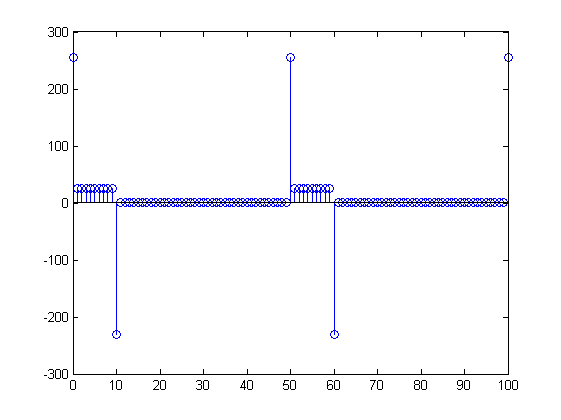
\includegraphics[width=0.4\textwidth]{content/5ww.png}}
	\subfloat[][y]{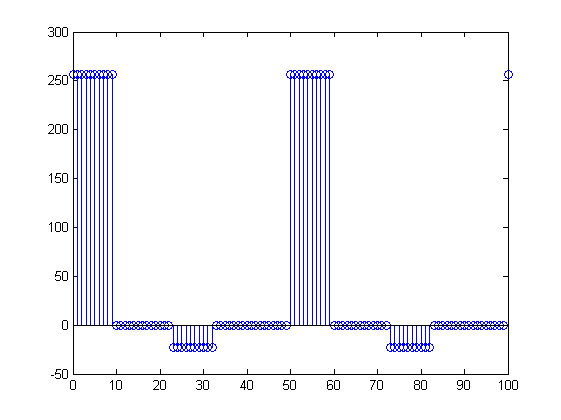
\includegraphics[width=0.4\textwidth]{content/5yy.png}}
  \caption{Stemplot van w en de benadering van w van x}
  \label{fig:opgave5}
\end{figure}
\section{Opgave 6}
In figuur \ref{fig:opgave6}
\begin{figure}[h]
  \centering
 	\subfloat[][x]{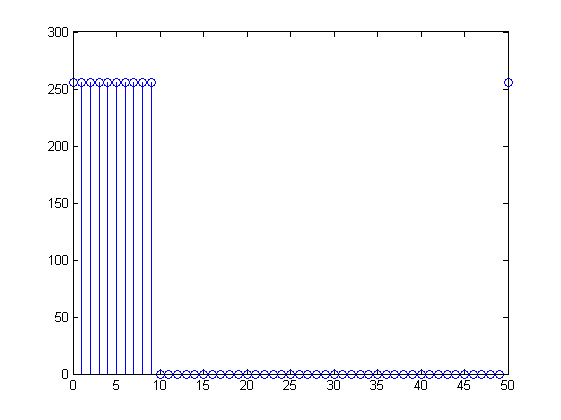
\includegraphics[width=0.4\textwidth]{content/6xx.png}}
	\subfloat[][y]{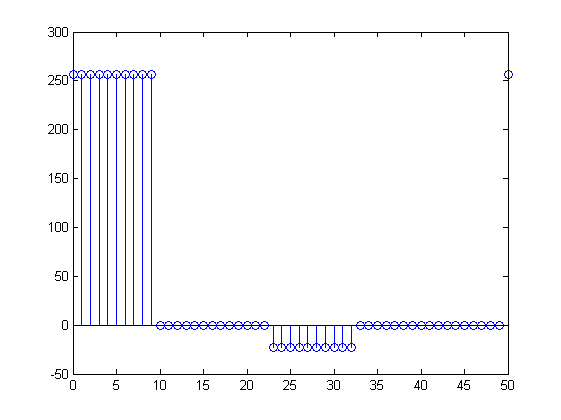
\includegraphics[width=0.4\textwidth]{content/6yy.png}}
	\subfloat[][x-y]{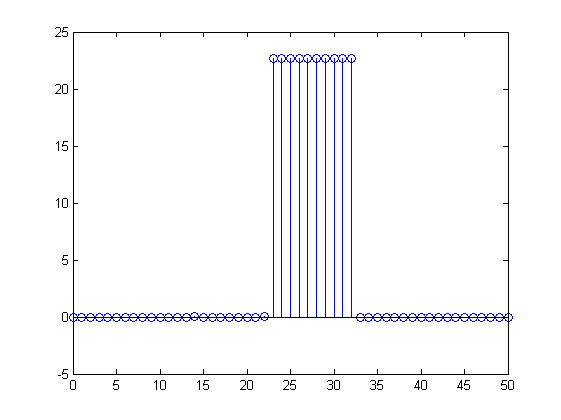
\includegraphics[width=0.4\textwidth]{content/6.png}}
  \caption{!!!!!!!!!}
  \label{fig:opgave6}
\end{figure}

\section{Opgave 7}
De waarde van r wordt bepaald door de sterkte die we aan de echo toekennen, het is immers de amplitude van het signaal P tijdeenheden terug dus: $r = 0.9$. P is de tijdverschuiving van de echo uigedrukt in tijdseenheden van de sample frequentie dus $p = \delta~t*f_s = 8000 * 0.2 = 1600$.

\section{Opgave 8}
De echo van een signaal kan met een FIR filter met convolutie $[1, 0_1 .. 0_p-1, 0.9]$ gemaakt worden. In matlab wordt het nieuwe signaal yy uit bronsignaal x2 berekend: $yy = conv(x2, [1 zeros(1,8000*0.2 - 1) 0.9]);$. Het oorspronkelijke signaal x2 en gefilterd signaal yy zijn uitgezet in figuur \ref{fig:opgave8}.
\begin{figure}[h]
  \centering
 	\subfloat[][x2]{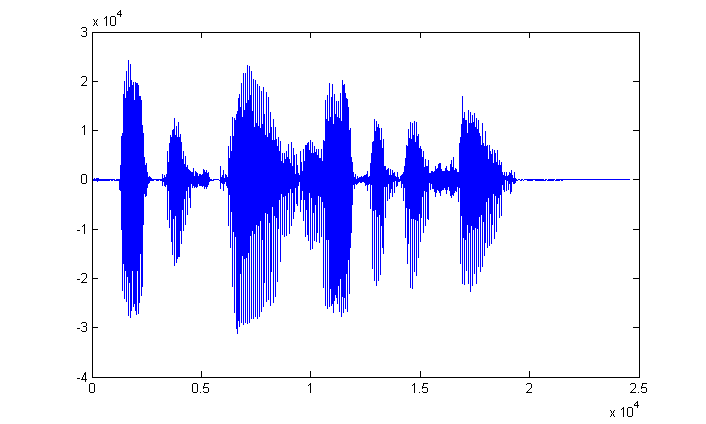
\includegraphics[width=0.4\textwidth]{content/8x2.png}}
	\subfloat[][yy]{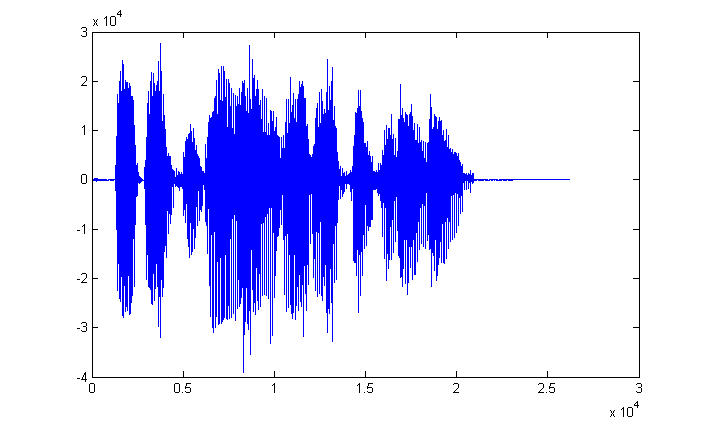
\includegraphics[width=0.4\textwidth]{content/8yy.png}}
  \caption{Het orginele signaal x2 verkregen uit functie labdat.mat en het signaal met echo yy}
  \label{fig:opgave8}
\end{figure}

\end{document}